\begin{frame}
\frametitle{Learning network protocols despite imperfect assumptions}
\begin{centering}
Can we design protocols to be forwards-compatible with higher link speeds?
\end{centering}
\end{frame}


\begin{frame}
\frametitle{Forwards compatibility with future link speeds}
\begin{centering}

\noindent \only<1>{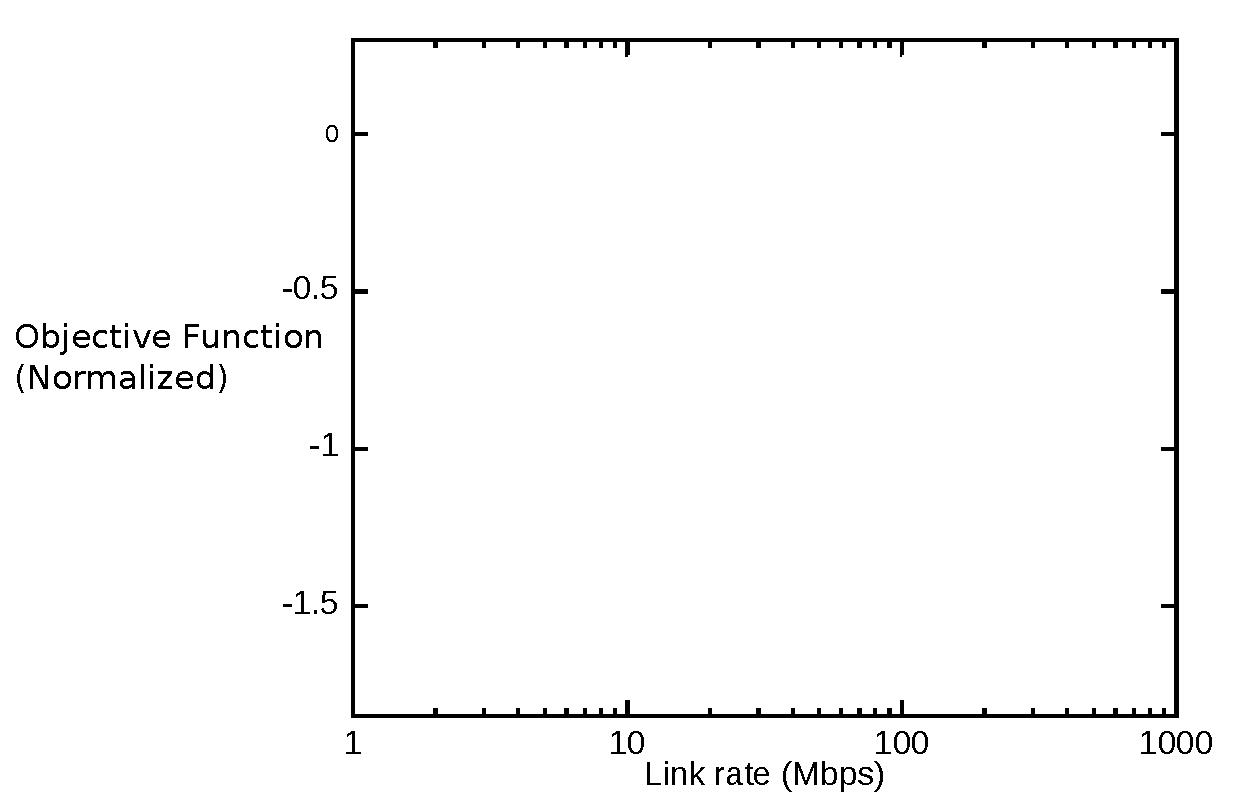
\includegraphics[width=3.1 in]{oprange-base.pdf}}\only<2>{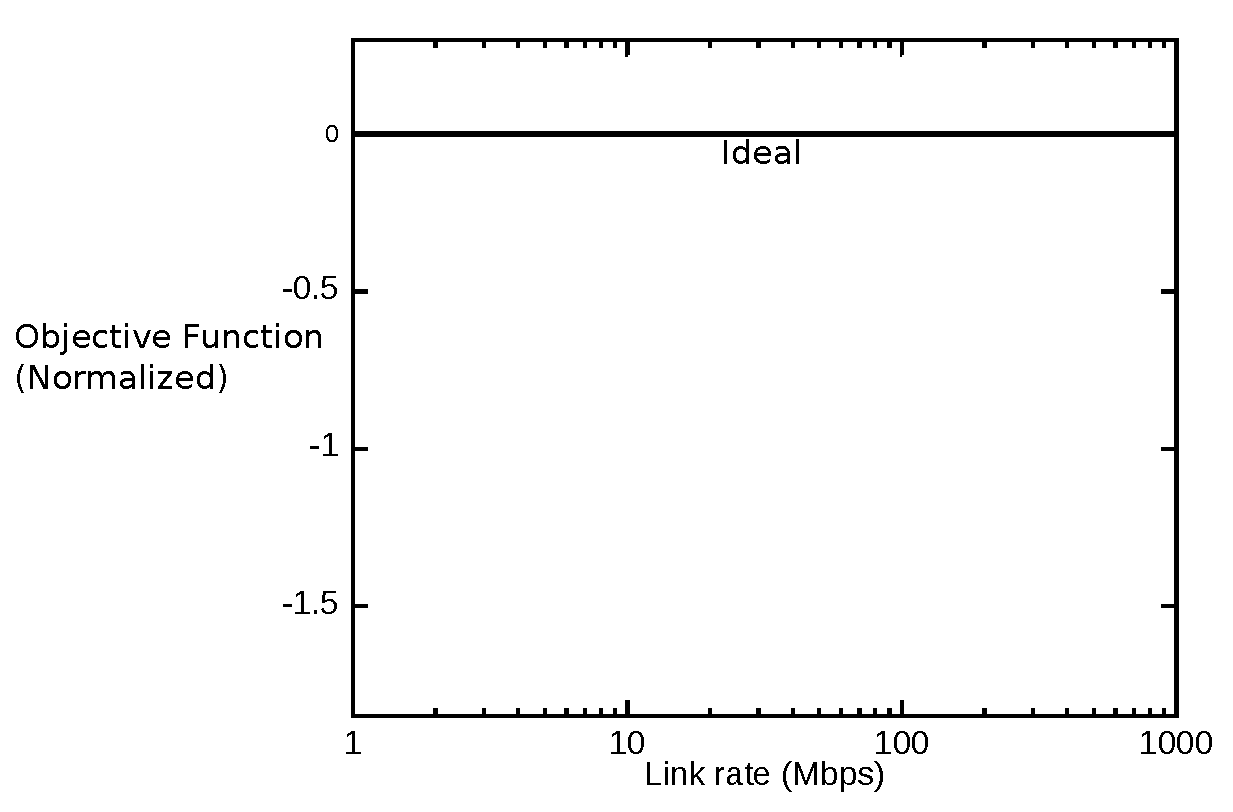
\includegraphics[width=3.1 in]{oprange-omniscient.pdf}}\only<3>{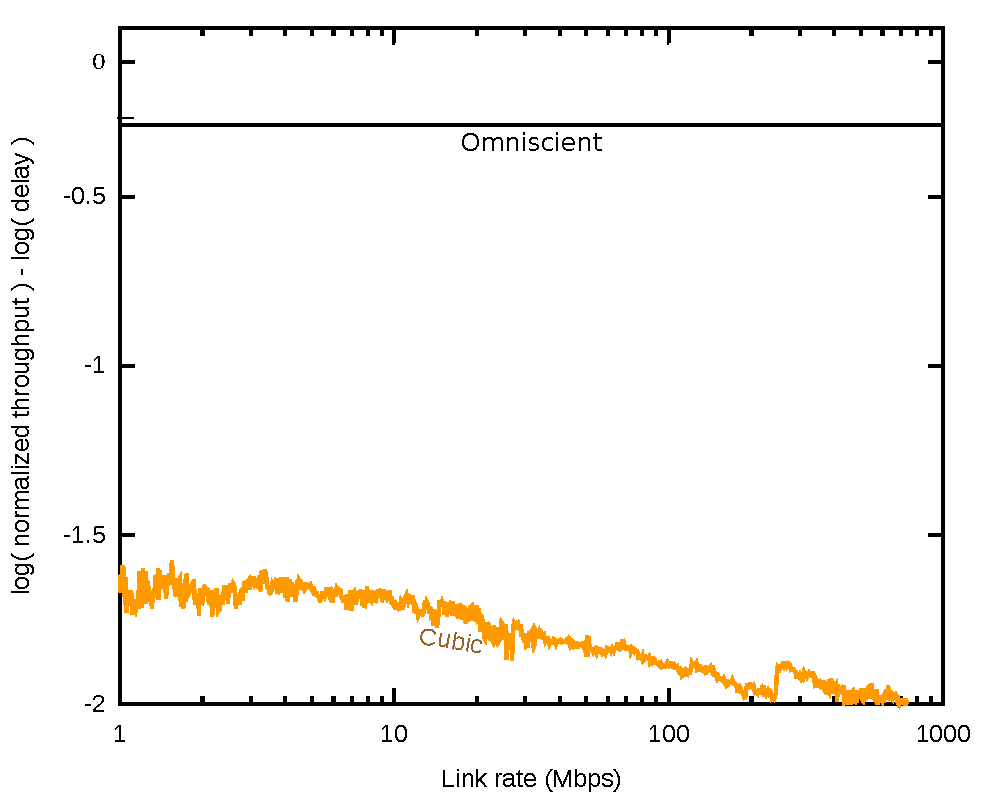
\includegraphics[width=3.1 in]{oprange-cubic.pdf}}\only<4>{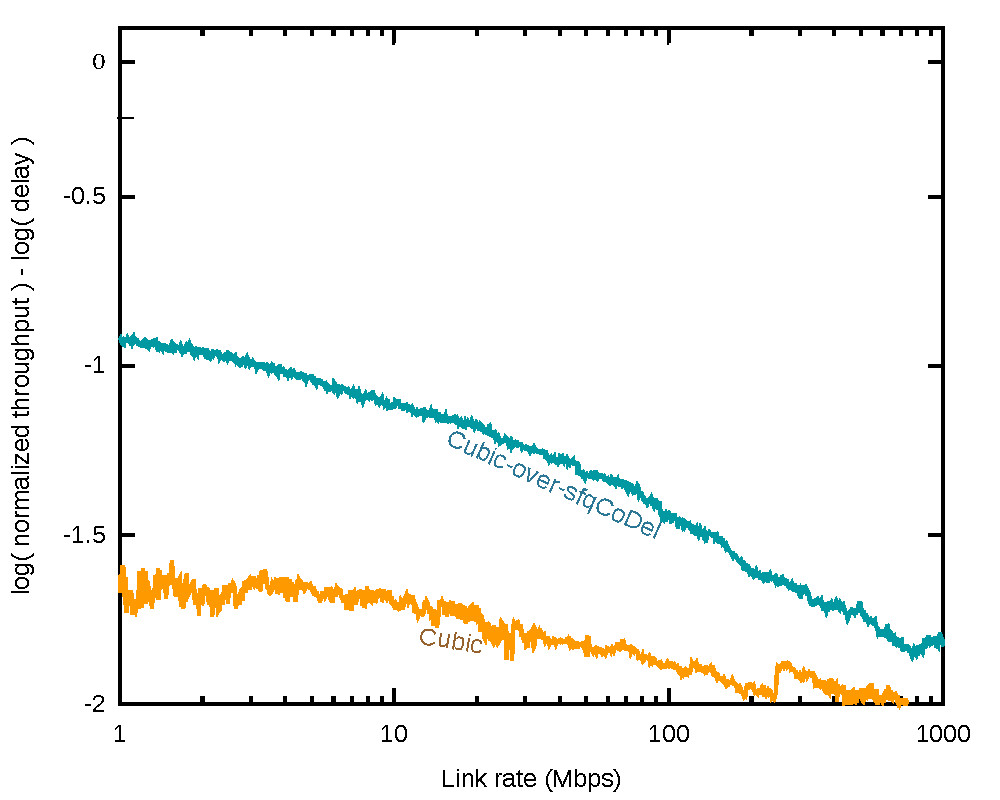
\includegraphics[width=3.1 in]{oprange-codel.pdf}}\only<5>{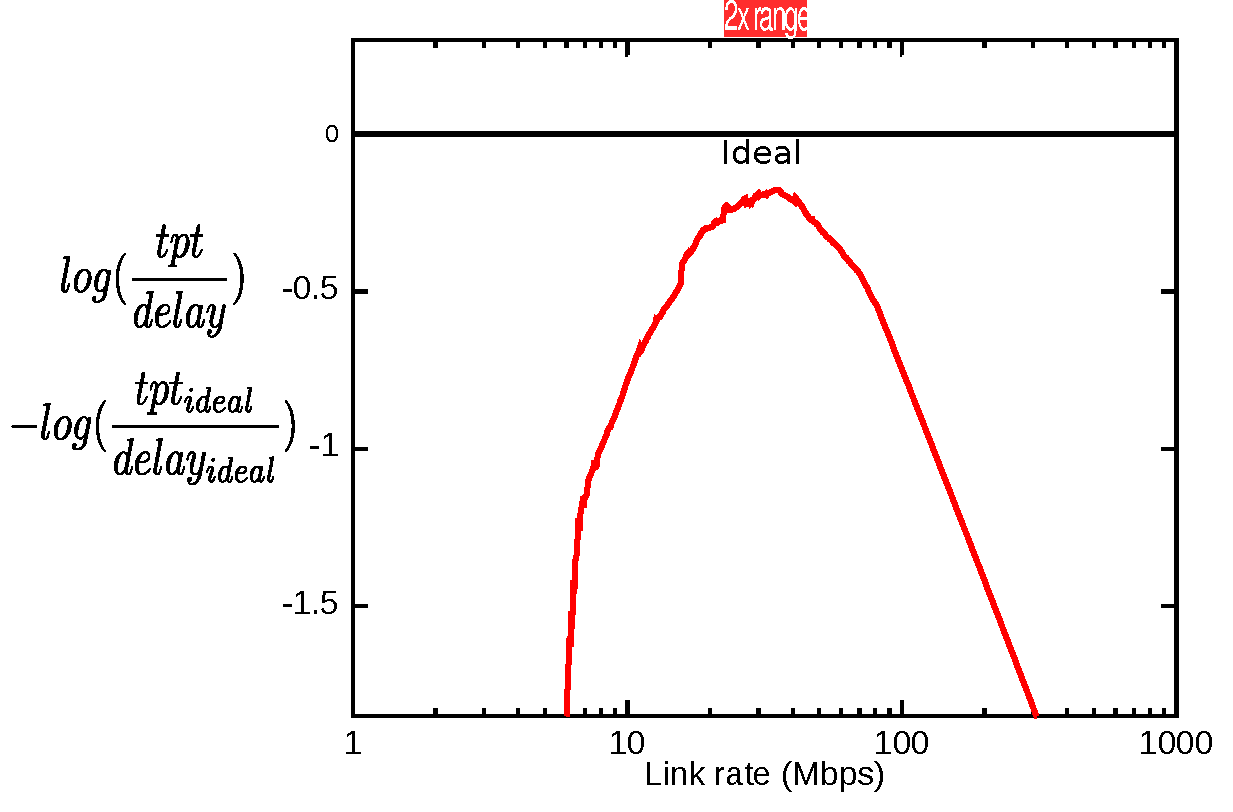
\includegraphics[width=3.1 in]{oprange-2x.pdf}}\only<6>{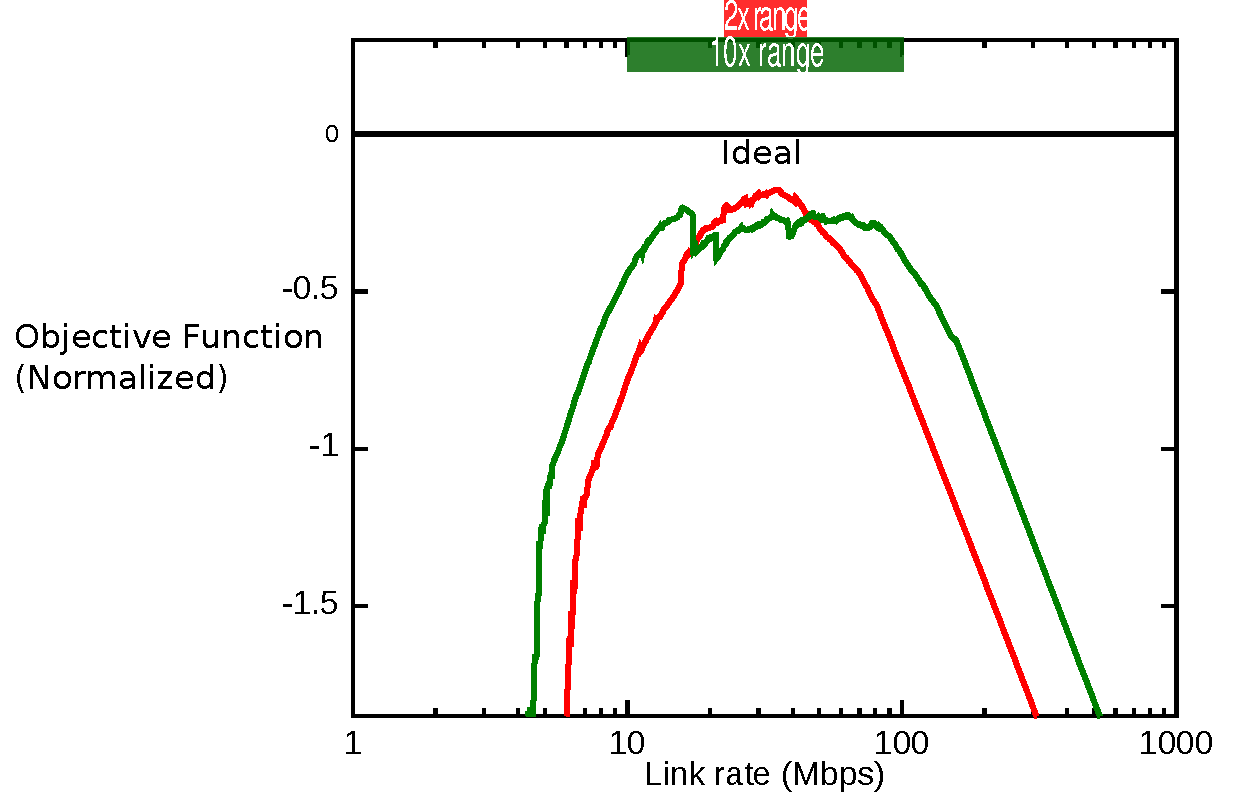
\includegraphics[width=3.1 in]{oprange-10x.pdf}}\only<7>{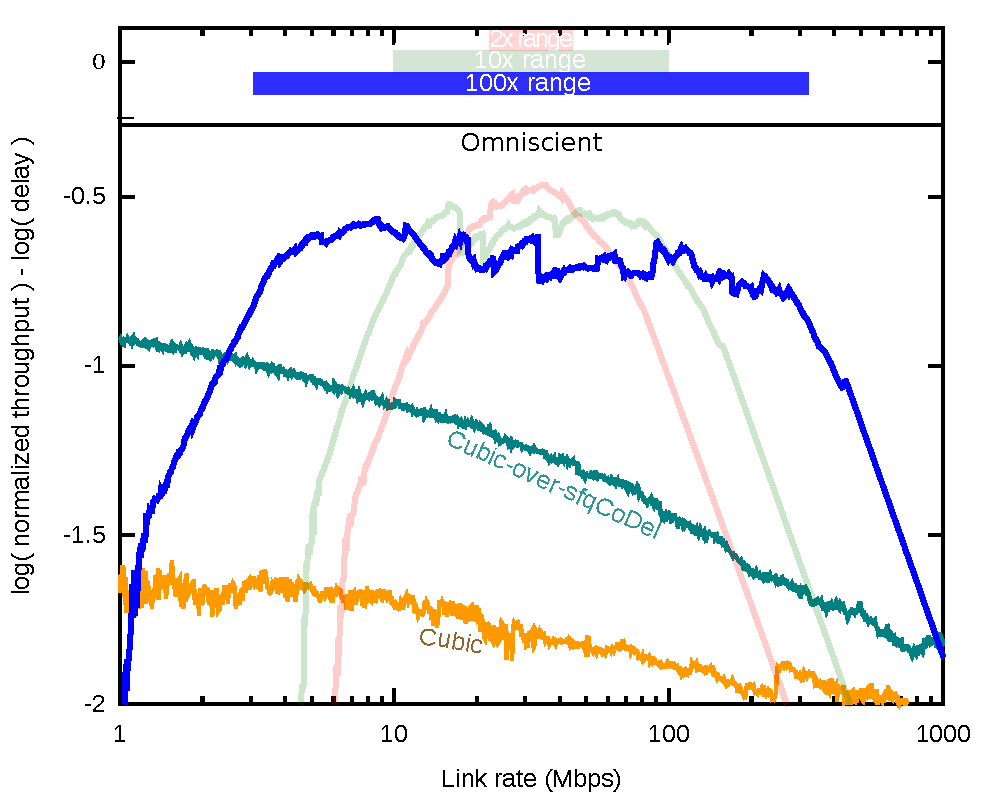
\includegraphics[width=3.1 in]{oprange-100x.pdf}}\only<8>{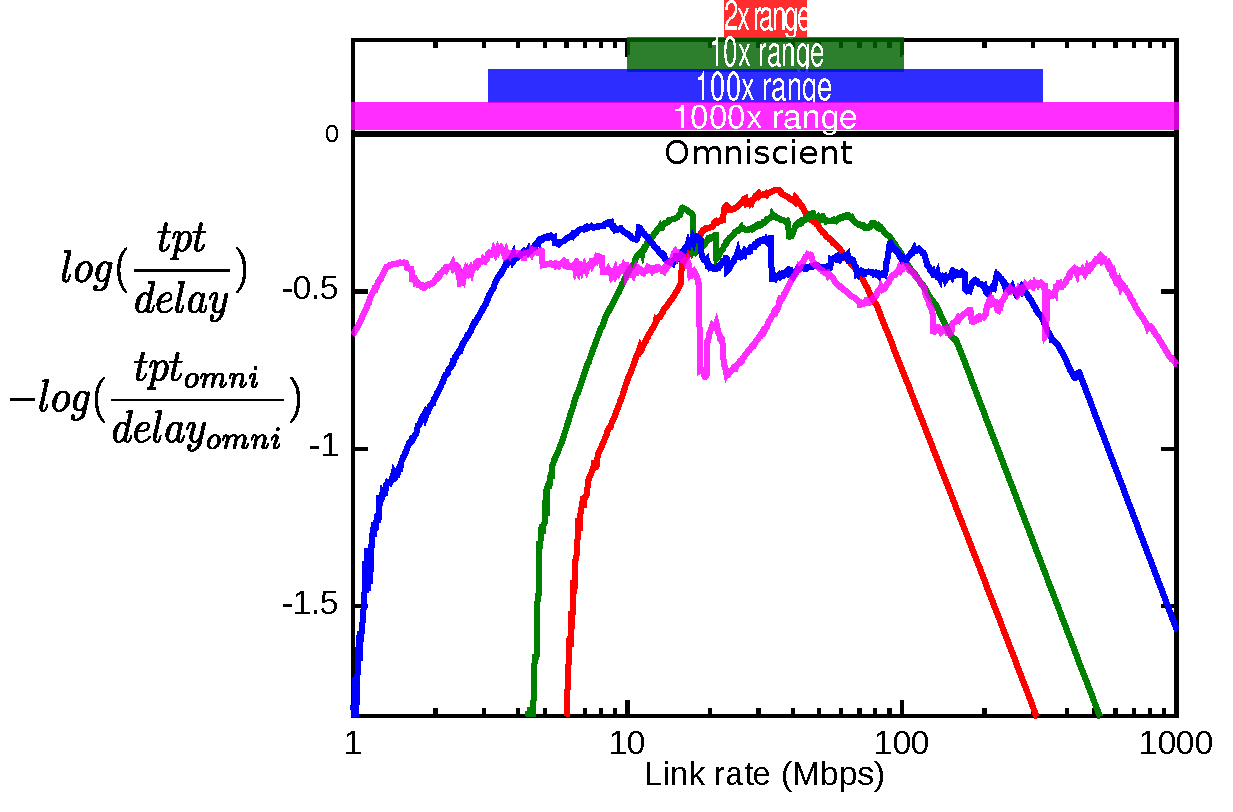
\includegraphics[width=3.1 in]{oprange-1000x.pdf}}

\only<9>{Only weak evidence of a performance-generality tradeoff}

\end{centering}
\end{frame}
